%Lualatex+needs P22UndergroundCYBookSC.tt and P22-Underground-Reg.ttf
\documentclass[
coverheight=9in,
coverwidth=6in,
spinewidth=0.515in,
bleedwidth=.125in,%.125in,
marklength=0in,
markcolor=black]{bookcover}

\usepackage{xcolor}
\usepackage{background}
\usepackage{blindtext}
\usepackage{fontspec}

\newbookcoverpart{pfront}{
\setpartposx{\marklength+\bleedwidth+\spinewidth+\coverwidth+6mm}
\setpartposy{\marklength+\bleedwidth+6mm}\setpartheight{\coverheight-12mm}
\setpartwidth{\coverwidth-12mm}
\settrimmedpart{0mm}{0mm}{0pt}{0pt}
}

\newbookcoverpart{pback}{
\setpartposx{\marklength+\bleedwidth+6mm}
\setpartposy{\marklength+\bleedwidth+6mm}\setpartheight{\coverheight-12mm}
\setpartwidth{\coverwidth-12mm}
\settrimmedpart{0mm}{0mm}{0pt}{0pt}
}

\begin{document}

\begin{bookcover}

\definecolor{textcolor}{HTML}{FFFFFF}

\bookcovercomponent{normal}{bg whole}{
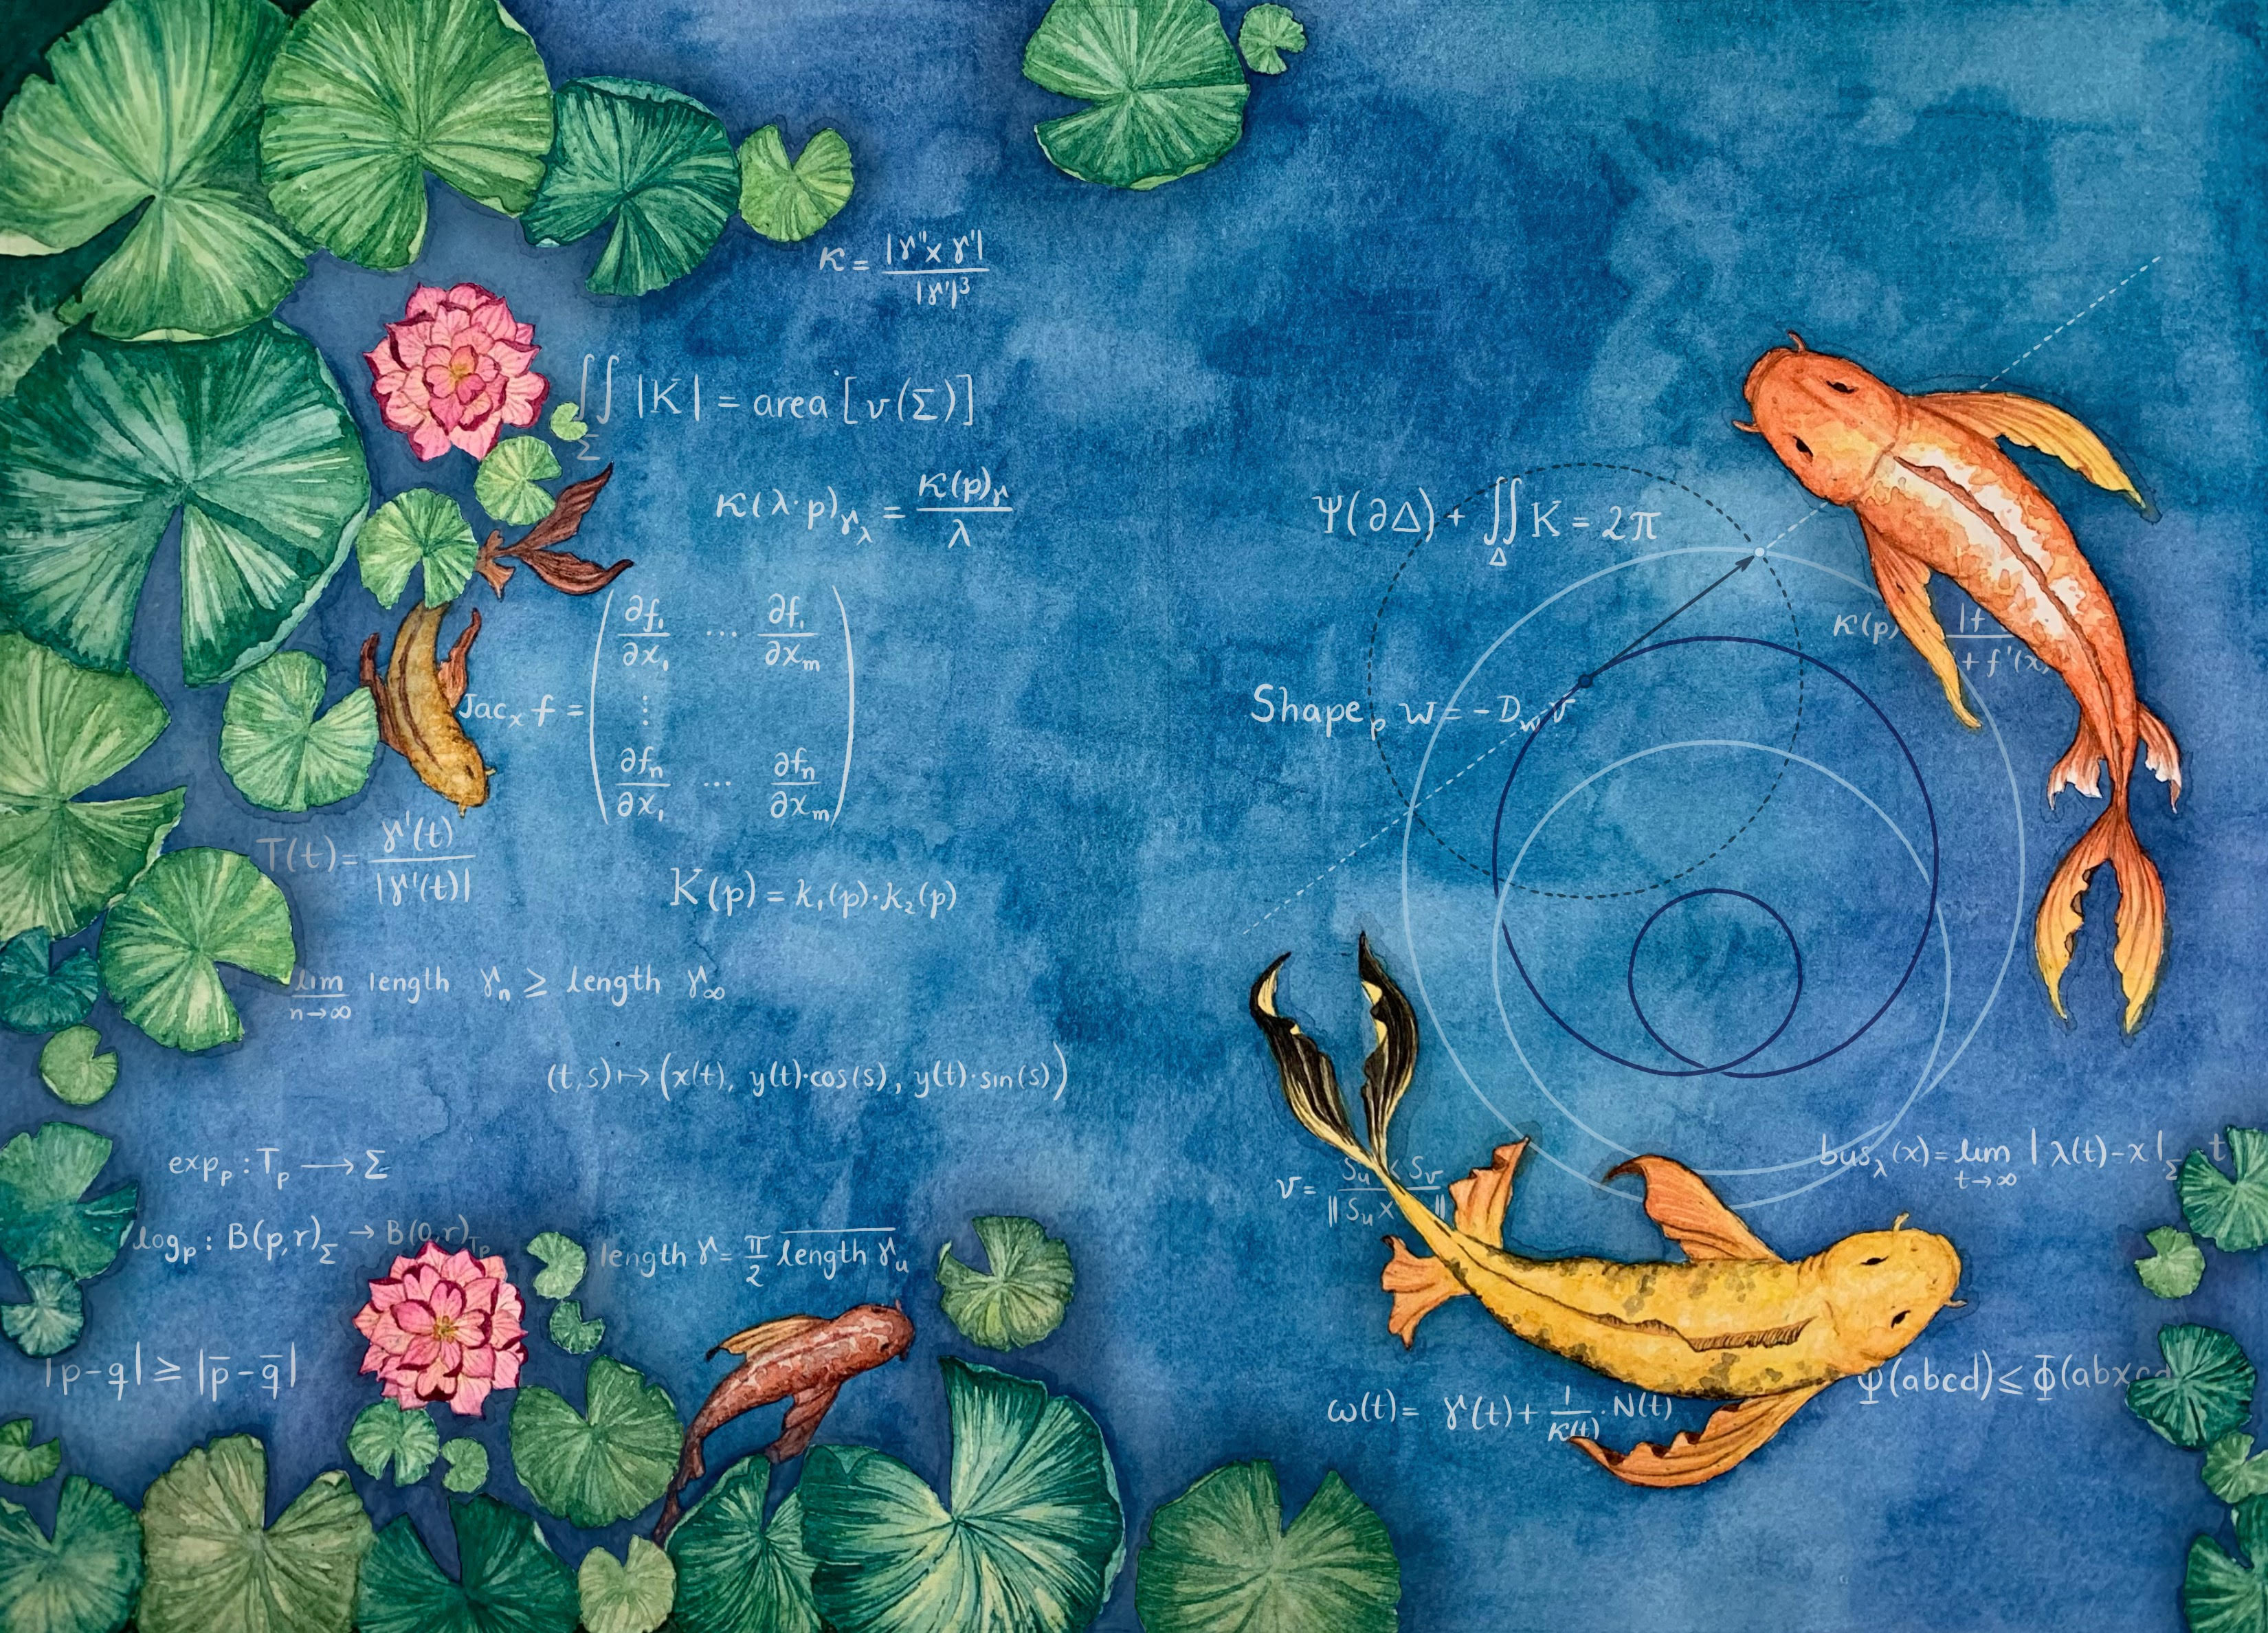
\includegraphics[width=.35cm+\textwidth]{drawing}
\vfill
}

\setmainfont{P22-Underground-Reg}

\bookcovercomponent{center}{spine}
{\rotatebox[origin=c]{-90}{
\color{textcolor}
\fontsize{18}{25}\selectfont
WHAT IS DIFFERENTIAL GEOMETRY?\qquad  CURVES AND SURFACES}}


\bookcovercomponent{normal}{pfront}{
\begin{center}
{\color{textcolor}\fontsize{23}{28}\selectfont
WHAT IS DIFFERENTIAL GEOMETRY?\\[5mm]
}
{{\color{textcolor}\fontsize{34}{28}\selectfont
CURVES AND SURFACES}\hskip-1mm
}
\end{center}
\vfill
\begin{center}
{\color{textcolor}\fontsize{17}{28}\selectfont
\ Anton Petrunin and Sergio Zamora Barrera
}
\end{center}
}

\bookcovercomponent{normal}{pback}{
\begin{flushleft}
\parbox{.35\textwidth}{
\color{textcolor}\fontsize{16}{18}\selectfont
These notes are designed for those who either plan to work in differential geometry,
or at least want to have a good reason not to do~it.}
\end{flushleft}
\vfill
\begin{flushleft}
{\color{textcolor}\fontsize{15}{28}\selectfont
arXiv:2012.11814v5\\
github.com/anton-petrunin/gauss}
\end{flushleft}
}
\end{bookcover}

\end{document}
